% Options for packages loaded elsewhere
\PassOptionsToPackage{unicode}{hyperref}
\PassOptionsToPackage{hyphens}{url}
%
\documentclass[
]{article}
\usepackage{amsmath,amssymb}
\usepackage{iftex}
\ifPDFTeX
  \usepackage[T1]{fontenc}
  \usepackage[utf8]{inputenc}
  \usepackage{textcomp} % provide euro and other symbols
\else % if luatex or xetex
  \usepackage{unicode-math} % this also loads fontspec
  \defaultfontfeatures{Scale=MatchLowercase}
  \defaultfontfeatures[\rmfamily]{Ligatures=TeX,Scale=1}
\fi
\usepackage{lmodern}
\ifPDFTeX\else
  % xetex/luatex font selection
\fi
% Use upquote if available, for straight quotes in verbatim environments
\IfFileExists{upquote.sty}{\usepackage{upquote}}{}
\IfFileExists{microtype.sty}{% use microtype if available
  \usepackage[]{microtype}
  \UseMicrotypeSet[protrusion]{basicmath} % disable protrusion for tt fonts
}{}
\makeatletter
\@ifundefined{KOMAClassName}{% if non-KOMA class
  \IfFileExists{parskip.sty}{%
    \usepackage{parskip}
  }{% else
    \setlength{\parindent}{0pt}
    \setlength{\parskip}{6pt plus 2pt minus 1pt}}
}{% if KOMA class
  \KOMAoptions{parskip=half}}
\makeatother
\usepackage{xcolor}
\usepackage[margin=1in]{geometry}
\usepackage{color}
\usepackage{fancyvrb}
\newcommand{\VerbBar}{|}
\newcommand{\VERB}{\Verb[commandchars=\\\{\}]}
\DefineVerbatimEnvironment{Highlighting}{Verbatim}{commandchars=\\\{\}}
% Add ',fontsize=\small' for more characters per line
\usepackage{framed}
\definecolor{shadecolor}{RGB}{248,248,248}
\newenvironment{Shaded}{\begin{snugshade}}{\end{snugshade}}
\newcommand{\AlertTok}[1]{\textcolor[rgb]{0.94,0.16,0.16}{#1}}
\newcommand{\AnnotationTok}[1]{\textcolor[rgb]{0.56,0.35,0.01}{\textbf{\textit{#1}}}}
\newcommand{\AttributeTok}[1]{\textcolor[rgb]{0.13,0.29,0.53}{#1}}
\newcommand{\BaseNTok}[1]{\textcolor[rgb]{0.00,0.00,0.81}{#1}}
\newcommand{\BuiltInTok}[1]{#1}
\newcommand{\CharTok}[1]{\textcolor[rgb]{0.31,0.60,0.02}{#1}}
\newcommand{\CommentTok}[1]{\textcolor[rgb]{0.56,0.35,0.01}{\textit{#1}}}
\newcommand{\CommentVarTok}[1]{\textcolor[rgb]{0.56,0.35,0.01}{\textbf{\textit{#1}}}}
\newcommand{\ConstantTok}[1]{\textcolor[rgb]{0.56,0.35,0.01}{#1}}
\newcommand{\ControlFlowTok}[1]{\textcolor[rgb]{0.13,0.29,0.53}{\textbf{#1}}}
\newcommand{\DataTypeTok}[1]{\textcolor[rgb]{0.13,0.29,0.53}{#1}}
\newcommand{\DecValTok}[1]{\textcolor[rgb]{0.00,0.00,0.81}{#1}}
\newcommand{\DocumentationTok}[1]{\textcolor[rgb]{0.56,0.35,0.01}{\textbf{\textit{#1}}}}
\newcommand{\ErrorTok}[1]{\textcolor[rgb]{0.64,0.00,0.00}{\textbf{#1}}}
\newcommand{\ExtensionTok}[1]{#1}
\newcommand{\FloatTok}[1]{\textcolor[rgb]{0.00,0.00,0.81}{#1}}
\newcommand{\FunctionTok}[1]{\textcolor[rgb]{0.13,0.29,0.53}{\textbf{#1}}}
\newcommand{\ImportTok}[1]{#1}
\newcommand{\InformationTok}[1]{\textcolor[rgb]{0.56,0.35,0.01}{\textbf{\textit{#1}}}}
\newcommand{\KeywordTok}[1]{\textcolor[rgb]{0.13,0.29,0.53}{\textbf{#1}}}
\newcommand{\NormalTok}[1]{#1}
\newcommand{\OperatorTok}[1]{\textcolor[rgb]{0.81,0.36,0.00}{\textbf{#1}}}
\newcommand{\OtherTok}[1]{\textcolor[rgb]{0.56,0.35,0.01}{#1}}
\newcommand{\PreprocessorTok}[1]{\textcolor[rgb]{0.56,0.35,0.01}{\textit{#1}}}
\newcommand{\RegionMarkerTok}[1]{#1}
\newcommand{\SpecialCharTok}[1]{\textcolor[rgb]{0.81,0.36,0.00}{\textbf{#1}}}
\newcommand{\SpecialStringTok}[1]{\textcolor[rgb]{0.31,0.60,0.02}{#1}}
\newcommand{\StringTok}[1]{\textcolor[rgb]{0.31,0.60,0.02}{#1}}
\newcommand{\VariableTok}[1]{\textcolor[rgb]{0.00,0.00,0.00}{#1}}
\newcommand{\VerbatimStringTok}[1]{\textcolor[rgb]{0.31,0.60,0.02}{#1}}
\newcommand{\WarningTok}[1]{\textcolor[rgb]{0.56,0.35,0.01}{\textbf{\textit{#1}}}}
\usepackage{graphicx}
\makeatletter
\def\maxwidth{\ifdim\Gin@nat@width>\linewidth\linewidth\else\Gin@nat@width\fi}
\def\maxheight{\ifdim\Gin@nat@height>\textheight\textheight\else\Gin@nat@height\fi}
\makeatother
% Scale images if necessary, so that they will not overflow the page
% margins by default, and it is still possible to overwrite the defaults
% using explicit options in \includegraphics[width, height, ...]{}
\setkeys{Gin}{width=\maxwidth,height=\maxheight,keepaspectratio}
% Set default figure placement to htbp
\makeatletter
\def\fps@figure{htbp}
\makeatother
\setlength{\emergencystretch}{3em} % prevent overfull lines
\providecommand{\tightlist}{%
  \setlength{\itemsep}{0pt}\setlength{\parskip}{0pt}}
\setcounter{secnumdepth}{-\maxdimen} % remove section numbering
\ifLuaTeX
  \usepackage{selnolig}  % disable illegal ligatures
\fi
\usepackage{bookmark}
\IfFileExists{xurl.sty}{\usepackage{xurl}}{} % add URL line breaks if available
\urlstyle{same}
\hypersetup{
  pdftitle={Homework 1},
  pdfauthor={Aaron Melcher},
  hidelinks,
  pdfcreator={LaTeX via pandoc}}

\title{Homework 1}
\author{Aaron Melcher}
\date{2024-09-30}

\begin{document}
\maketitle

\begin{verbatim}
## -- Attaching core tidyverse packages ------------------------ tidyverse 2.0.0 --
## v dplyr     1.1.4     v readr     2.1.5
## v forcats   1.0.0     v stringr   1.5.1
## v ggplot2   3.5.1     v tibble    3.2.1
## v lubridate 1.9.3     v tidyr     1.3.1
## v purrr     1.0.2     
## -- Conflicts ------------------------------------------ tidyverse_conflicts() --
## x dplyr::filter() masks stats::filter()
## x dplyr::lag()    masks stats::lag()
## i Use the conflicted package (<http://conflicted.r-lib.org/>) to force all conflicts to become errors
\end{verbatim}

\#{[}NYC Flights{]}

\begin{Shaded}
\begin{Highlighting}[]
\FunctionTok{library}\NormalTok{(nycflights13)}
\NormalTok{flights }\SpecialCharTok{|\textgreater{}} \FunctionTok{select}\NormalTok{(carrier, air\_time, distance)}
\end{Highlighting}
\end{Shaded}

\begin{verbatim}
## # A tibble: 336,776 x 3
##    carrier air_time distance
##    <chr>      <dbl>    <dbl>
##  1 UA           227     1400
##  2 UA           227     1416
##  3 AA           160     1089
##  4 B6           183     1576
##  5 DL           116      762
##  6 UA           150      719
##  7 B6           158     1065
##  8 EV            53      229
##  9 B6           140      944
## 10 AA           138      733
## # i 336,766 more rows
\end{verbatim}

\#\#Part A

\begin{Shaded}
\begin{Highlighting}[]
\NormalTok{flights }\OtherTok{\textless{}{-}} \FunctionTok{mutate}\NormalTok{(flights,}
  \AttributeTok{speed =}\NormalTok{ distance }\SpecialCharTok{/}\NormalTok{ air\_time}
\NormalTok{)}
\NormalTok{flights}
\end{Highlighting}
\end{Shaded}

\begin{verbatim}
## # A tibble: 336,776 x 20
##     year month   day dep_time sched_dep_time dep_delay arr_time sched_arr_time
##    <int> <int> <int>    <int>          <int>     <dbl>    <int>          <int>
##  1  2013     1     1      517            515         2      830            819
##  2  2013     1     1      533            529         4      850            830
##  3  2013     1     1      542            540         2      923            850
##  4  2013     1     1      544            545        -1     1004           1022
##  5  2013     1     1      554            600        -6      812            837
##  6  2013     1     1      554            558        -4      740            728
##  7  2013     1     1      555            600        -5      913            854
##  8  2013     1     1      557            600        -3      709            723
##  9  2013     1     1      557            600        -3      838            846
## 10  2013     1     1      558            600        -2      753            745
## # i 336,766 more rows
## # i 12 more variables: arr_delay <dbl>, carrier <chr>, flight <int>,
## #   tailnum <chr>, origin <chr>, dest <chr>, air_time <dbl>, distance <dbl>,
## #   hour <dbl>, minute <dbl>, time_hour <dttm>, speed <dbl>
\end{verbatim}

\#\#Part B

\begin{Shaded}
\begin{Highlighting}[]
\FunctionTok{ggplot}\NormalTok{(flights, }\FunctionTok{aes}\NormalTok{(carrier, speed)) }\SpecialCharTok{+}
  \FunctionTok{geom\_boxplot}\NormalTok{()}
\end{Highlighting}
\end{Shaded}

\begin{verbatim}
## Warning: Removed 9430 rows containing non-finite outside the scale range
## (`stat_boxplot()`).
\end{verbatim}

\includegraphics{hmwk1_files/figure-latex/unnamed-chunk-4-1.pdf}

The boxplot above provides a very basic analysis of the average speed of
each carrier. With this, we are able to see carrier `HA' has the highest
average speed of any of the carriers. Even though some of the carriers
do have higher `highs', HA still on average is faster than the others.

\#{[}London Olympics{]}

\begin{Shaded}
\begin{Highlighting}[]
\NormalTok{olympics }\OtherTok{\textless{}{-}} \FunctionTok{read\_csv}\NormalTok{(}\StringTok{"https://uwmadison.box.com/shared/static/rzw8h2x6dp5693gdbpgxaf2koqijo12l.csv"}\NormalTok{)}
\end{Highlighting}
\end{Shaded}

\#\#Part A/B

\begin{Shaded}
\begin{Highlighting}[]
\NormalTok{counts }\OtherTok{\textless{}{-}}\NormalTok{ olympics }\SpecialCharTok{|\textgreater{}}
  \FunctionTok{count}\NormalTok{(Sport)}

\NormalTok{olympics }\SpecialCharTok{|\textgreater{}}
  \FunctionTok{left\_join}\NormalTok{(counts) }\SpecialCharTok{|\textgreater{}}
  \FunctionTok{filter}\NormalTok{(n }\SpecialCharTok{\textgreater{}} \DecValTok{5}\NormalTok{) }\SpecialCharTok{|\textgreater{}}
  \FunctionTok{ggplot}\NormalTok{() }\SpecialCharTok{+}
  \FunctionTok{geom\_boxplot}\NormalTok{(}
    \FunctionTok{aes}\NormalTok{(Age, }\FunctionTok{reorder}\NormalTok{(Sport, Age, sd))}
\NormalTok{  )}
\end{Highlighting}
\end{Shaded}

\includegraphics{hmwk1_files/figure-latex/unnamed-chunk-6-1.pdf}

\#\#Part C

Average height(cm) among sports. See if there's a noticeable difference
in the height among athletes that participate in different sports.
Following the same idea as the age distribution, I created a
visualization on based on height.

\begin{Shaded}
\begin{Highlighting}[]
\NormalTok{olympics }\SpecialCharTok{|\textgreater{}}
  \FunctionTok{left\_join}\NormalTok{(counts) }\SpecialCharTok{|\textgreater{}}
  \FunctionTok{filter}\NormalTok{(n }\SpecialCharTok{\textgreater{}} \DecValTok{5}\NormalTok{) }\SpecialCharTok{|\textgreater{}}
  \FunctionTok{ggplot}\NormalTok{() }\SpecialCharTok{+}
  \FunctionTok{geom\_boxplot}\NormalTok{(}
    \FunctionTok{aes}\NormalTok{(}\StringTok{\textasciigrave{}}\AttributeTok{Height, cm}\StringTok{\textasciigrave{}}\NormalTok{, }\FunctionTok{reorder}\NormalTok{(Sport, }\StringTok{\textasciigrave{}}\AttributeTok{Height, cm}\StringTok{\textasciigrave{}}\NormalTok{, sd))}
\NormalTok{  )}
\end{Highlighting}
\end{Shaded}

\begin{verbatim}
## Warning: Removed 561 rows containing non-finite outside the scale range
## (`stat_boxplot()`).
\end{verbatim}

\includegraphics{hmwk1_files/figure-latex/unnamed-chunk-7-1.pdf}

There does not seem to be a very noticeable difference in height, except
in basketball, which does make sense.

\#{[}Pokemon{]}

\begin{Shaded}
\begin{Highlighting}[]
\NormalTok{pokemon }\OtherTok{\textless{}{-}} \FunctionTok{read\_csv}\NormalTok{(}\StringTok{"https://uwmadison.box.com/shared/static/hf5cmx3ew3ch0v6t0c2x56838er1lt2c.csv"}\NormalTok{)}
\end{Highlighting}
\end{Shaded}

\#\#Part A

\begin{Shaded}
\begin{Highlighting}[]
\NormalTok{pokemon }\OtherTok{\textless{}{-}} \FunctionTok{mutate}\NormalTok{(}
\NormalTok{  pokemon,}
  \StringTok{\textquotesingle{}attack{-}to{-}defense\textquotesingle{}} \OtherTok{=}\NormalTok{ Attack }\SpecialCharTok{/}\NormalTok{ Defense}
\NormalTok{)}
\NormalTok{pokemon }\SpecialCharTok{|\textgreater{}} \FunctionTok{select}\NormalTok{(}\StringTok{\textquotesingle{}attack{-}to{-}defense\textquotesingle{}}\NormalTok{)}
\end{Highlighting}
\end{Shaded}

\begin{verbatim}
## # A tibble: 800 x 1
##    `attack-to-defense`
##                  <dbl>
##  1               1    
##  2               0.984
##  3               0.988
##  4               0.813
##  5               1.21 
##  6               1.10 
##  7               1.08 
##  8               1.17 
##  9               1.33 
## 10               0.738
## # i 790 more rows
\end{verbatim}

\#\#Part B

\begin{Shaded}
\begin{Highlighting}[]
\NormalTok{pokemon }\OtherTok{\textless{}{-}}\NormalTok{ pokemon }\SpecialCharTok{|\textgreater{}}
  \FunctionTok{group\_by}\NormalTok{(type\_1) }\SpecialCharTok{|\textgreater{}}
  \FunctionTok{mutate}\NormalTok{(}\StringTok{\textasciigrave{}}\AttributeTok{attack{-}to{-}defense{-}median}\StringTok{\textasciigrave{}} \OtherTok{=} \FunctionTok{median}\NormalTok{(}\StringTok{\textasciigrave{}}\AttributeTok{attack{-}to{-}defense}\StringTok{\textasciigrave{}}\NormalTok{, }\AttributeTok{na.rm =} \ConstantTok{TRUE}\NormalTok{)) }\SpecialCharTok{|\textgreater{}}
  \FunctionTok{ungroup}\NormalTok{()}
\NormalTok{pokemon}
\end{Highlighting}
\end{Shaded}

\begin{verbatim}
## # A tibble: 800 x 14
##    Name      type_1 type_2 Total    HP Attack Defense speed_attack speed_defense
##    <chr>     <chr>  <chr>  <dbl> <dbl>  <dbl>   <dbl>        <dbl>         <dbl>
##  1 Bulbasaur Grass  Poison   318    45     49      49           65            65
##  2 Ivysaur   Grass  Poison   405    60     62      63           80            80
##  3 Venusaur  Grass  Poison   525    80     82      83          100           100
##  4 Venusaur~ Grass  Poison   625    80    100     123          122           120
##  5 Charmand~ Fire   <NA>     309    39     52      43           60            50
##  6 Charmele~ Fire   <NA>     405    58     64      58           80            65
##  7 Charizard Fire   Flying   534    78     84      78          109            85
##  8 Charizar~ Fire   Dragon   634    78    130     111          130            85
##  9 Charizar~ Fire   Flying   634    78    104      78          159           115
## 10 Squirtle  Water  <NA>     314    44     48      65           50            64
## # i 790 more rows
## # i 5 more variables: Speed <dbl>, Generation <dbl>, Legendary <lgl>,
## #   `attack-to-defense` <dbl>, `attack-to-defense-median` <dbl>
\end{verbatim}

\#\#Part C

\begin{Shaded}
\begin{Highlighting}[]
\NormalTok{pokemon}\SpecialCharTok{$}\NormalTok{type\_1 }\OtherTok{\textless{}{-}} \FunctionTok{reorder}\NormalTok{(pokemon}\SpecialCharTok{$}\NormalTok{type\_1, }\FunctionTok{desc}\NormalTok{(pokemon}\SpecialCharTok{$}\StringTok{\textasciigrave{}}\AttributeTok{attack{-}to{-}defense{-}median}\StringTok{\textasciigrave{}}\NormalTok{))}

\FunctionTok{ggplot}\NormalTok{(}
\NormalTok{  pokemon,}
  \FunctionTok{aes}\NormalTok{(}\StringTok{\textasciigrave{}}\AttributeTok{attack{-}to{-}defense}\StringTok{\textasciigrave{}}\NormalTok{)}
\NormalTok{  ) }\SpecialCharTok{+}
  \FunctionTok{geom\_dotplot}\NormalTok{() }\SpecialCharTok{+}
  \FunctionTok{facet\_wrap}\NormalTok{(}\StringTok{"type\_1"}\NormalTok{, }\AttributeTok{scales =} \StringTok{"free\_x"}\NormalTok{) }\SpecialCharTok{+}
  \FunctionTok{theme\_classic}\NormalTok{()}
\end{Highlighting}
\end{Shaded}

\includegraphics{hmwk1_files/figure-latex/unnamed-chunk-11-1.pdf}

\#\#Part D

An example dynamic plot could compare the stat totals of Pokemon based
on different factors. For example, we could see the difference based on
type or legendary status. This would answer how strong some types are or
how strong legendary Pokemon are compared to regular Pokemon. The user
would be able to select what facet they want to view and the query would
update how the stat totals are shown.

\#{[}Gene Expression Faceting{]}

\begin{Shaded}
\begin{Highlighting}[]
\NormalTok{genes }\OtherTok{\textless{}{-}} \FunctionTok{read\_csv}\NormalTok{(}\StringTok{"https://uwmadison.box.com/shared/static/dwzchdtfca33r0f6i055k2d0939onnlv.csv"}\NormalTok{)}
\FunctionTok{head}\NormalTok{(genes, }\DecValTok{3}\NormalTok{)}
\end{Highlighting}
\end{Shaded}

\begin{verbatim}
## # A tibble: 3 x 4
##   sample gene   time value
##    <dbl> <chr> <dbl> <dbl>
## 1      1 Pyy   0.677   103
## 2      1 Iapp  0.677     0
## 3      1 Chgb  0.677    86
\end{verbatim}

\#\#Part A

\begin{Shaded}
\begin{Highlighting}[]
\NormalTok{genes }\OtherTok{\textless{}{-}} \FunctionTok{mutate}\NormalTok{(genes,}
                \StringTok{\textquotesingle{}log(1 + value)\textquotesingle{}} \OtherTok{=} \FunctionTok{log}\NormalTok{(}\DecValTok{1} \SpecialCharTok{+}\NormalTok{ value)}
\NormalTok{                )}

\FunctionTok{ggplot}\NormalTok{(genes, }\FunctionTok{aes}\NormalTok{(}
  \AttributeTok{x =}\NormalTok{ time,}
  \AttributeTok{y =} \StringTok{\textasciigrave{}}\AttributeTok{log(1 + value)}\StringTok{\textasciigrave{}}\NormalTok{,}
  \AttributeTok{alpha =} \FloatTok{0.5}
\NormalTok{)) }\SpecialCharTok{+}
  \FunctionTok{geom\_point}\NormalTok{() }\SpecialCharTok{+}
  \FunctionTok{facet\_wrap}\NormalTok{(}\SpecialCharTok{\textasciitilde{}}\NormalTok{ gene) }\SpecialCharTok{+}
  \FunctionTok{theme\_bw}\NormalTok{()}
\end{Highlighting}
\end{Shaded}

\includegraphics{hmwk1_files/figure-latex/unnamed-chunk-13-1.pdf}

\#\#Part B One advantage of small multiples is being able to compare
multiple graphs one the same scale. This allows for comparisons between
different facets such as shown in the graph above.

One disadvantage of small multiples is trying to display large amounts
of data since too many graphs can be overwhelming and unweildy with lots
of different information.

\#\#Part C

\begin{Shaded}
\begin{Highlighting}[]
\NormalTok{gene\_groups }\OtherTok{\textless{}{-}}\NormalTok{ genes }\SpecialCharTok{|\textgreater{}}
\FunctionTok{group\_by}\NormalTok{(gene, }\AttributeTok{rounded\_time =} \FunctionTok{round}\NormalTok{(time, }\DecValTok{2}\NormalTok{)) }\SpecialCharTok{|\textgreater{}}
\FunctionTok{summarise}\NormalTok{(}\AttributeTok{mean\_value =} \FunctionTok{mean}\NormalTok{(value))}
\FunctionTok{head}\NormalTok{(gene\_groups, }\DecValTok{3}\NormalTok{)}
\end{Highlighting}
\end{Shaded}

\begin{verbatim}
## # A tibble: 3 x 3
## # Groups:   gene [1]
##   gene  rounded_time mean_value
##   <chr>        <dbl>      <dbl>
## 1 Cck           0        0     
## 2 Cck           0.01     0     
## 3 Cck           0.02     0.0652
\end{verbatim}

\#\#Part D

\begin{Shaded}
\begin{Highlighting}[]
\NormalTok{fitted\_values }\OtherTok{\textless{}{-}} \FunctionTok{read\_csv}\NormalTok{(}\StringTok{"https://go.wisc.edu/x678hu"}\NormalTok{)}
\FunctionTok{head}\NormalTok{(fitted\_values, }\DecValTok{3}\NormalTok{)}
\end{Highlighting}
\end{Shaded}

\begin{verbatim}
## # A tibble: 3 x 4
##   gene   time     mu sigma
##   <chr> <dbl>  <dbl> <dbl>
## 1 Pyy   0.677  52.8   3.17
## 2 Pyy   0.432   2.47  1.23
## 3 Pyy   0.749 112.    1.95
\end{verbatim}

\begin{Shaded}
\begin{Highlighting}[]
\FunctionTok{ggplot}\NormalTok{(genes, }\FunctionTok{aes}\NormalTok{(}
  \AttributeTok{x =}\NormalTok{ time,}
  \AttributeTok{y =} \StringTok{\textasciigrave{}}\AttributeTok{log(1 + value)}\StringTok{\textasciigrave{}}\NormalTok{,}
  \AttributeTok{alpha =} \FloatTok{0.5}
\NormalTok{)) }\SpecialCharTok{+}
  \FunctionTok{geom\_point}\NormalTok{() }\SpecialCharTok{+}
  \FunctionTok{geom\_line}\NormalTok{(}
    \AttributeTok{data =}\NormalTok{ fitted\_values,}
    \FunctionTok{aes}\NormalTok{(}
      \AttributeTok{x =}\NormalTok{ time,}
      \AttributeTok{y =} \FunctionTok{log}\NormalTok{(mu),}
      \AttributeTok{color =} \StringTok{\textquotesingle{}red\textquotesingle{}}
\NormalTok{    ),}
    \AttributeTok{size =} \FloatTok{1.5}
\NormalTok{  ) }\SpecialCharTok{+}
  \FunctionTok{facet\_wrap}\NormalTok{(}\SpecialCharTok{\textasciitilde{}}\NormalTok{ gene) }\SpecialCharTok{+}
  \FunctionTok{theme\_bw}\NormalTok{()}
\end{Highlighting}
\end{Shaded}

\begin{verbatim}
## Warning: Using `size` aesthetic for lines was deprecated in ggplot2 3.4.0.
## i Please use `linewidth` instead.
## This warning is displayed once every 8 hours.
## Call `lifecycle::last_lifecycle_warnings()` to see where this warning was
## generated.
\end{verbatim}

\includegraphics{hmwk1_files/figure-latex/unnamed-chunk-16-1.pdf}

\#{[}Visual Redesign{]}

\#\#Part A Here is the code for a very basic visualization that was done
in a past Stats class:

\begin{Shaded}
\begin{Highlighting}[]
\NormalTok{n\_df }\OtherTok{=} \FunctionTok{read.csv}\NormalTok{(}\StringTok{"nile.csv"}\NormalTok{)}

\FunctionTok{ggplot}\NormalTok{(n\_df) }\SpecialCharTok{+}
  \FunctionTok{geom\_point}\NormalTok{(}\FunctionTok{aes}\NormalTok{(}
    \AttributeTok{x =}\NormalTok{ Year,}
    \AttributeTok{y =}\NormalTok{ Flow}
\NormalTok{  )) }\SpecialCharTok{+}
  \FunctionTok{xlab}\NormalTok{(}\StringTok{"Year"}\NormalTok{) }\SpecialCharTok{+}
  \FunctionTok{ylab}\NormalTok{(}\StringTok{"Flow (10\textquotesingle{}s of Millions cubic meters)"}\NormalTok{)}
\end{Highlighting}
\end{Shaded}

\includegraphics{hmwk1_files/figure-latex/unnamed-chunk-17-1.pdf}

\#\#Part B The main takeaways from the above graph are the overall
decline in water flow over the time period. This is somewhat consistent
from the visualization as there really isn't an intended message and the
interpretation of the data is left up to the viewer.

\#\#Part C The visualization is legible but hard to draw any ideas from
as there is any additional visualization provided to help highlight more
information. The dataset itself isn't super in-depth but additional
visual elements can help with providing more in-depth analysis.

\#\#Part D Here is a new visualization that uses the original design but
adds a basic overlay to better highlight the information I want the
viewer to know. With the limited data, there isn't too much more that
can be visualized.

\begin{Shaded}
\begin{Highlighting}[]
\FunctionTok{ggplot}\NormalTok{(n\_df, }
       \FunctionTok{aes}\NormalTok{(}
         \AttributeTok{x =}\NormalTok{ Year, }
         \AttributeTok{y =}\NormalTok{ Flow)}
\NormalTok{       ) }\SpecialCharTok{+}
  \FunctionTok{geom\_point}\NormalTok{() }\SpecialCharTok{+}
  \FunctionTok{geom\_smooth}\NormalTok{(}
    \AttributeTok{method =} \StringTok{"lm"}\NormalTok{, }
    \AttributeTok{se =} \ConstantTok{FALSE}\NormalTok{, }
    \AttributeTok{color =} \StringTok{"red"}\NormalTok{, }
    \AttributeTok{size =} \DecValTok{1}
\NormalTok{    ) }\SpecialCharTok{+}
  \FunctionTok{xlab}\NormalTok{(}\StringTok{"Year"}\NormalTok{) }\SpecialCharTok{+}
  \FunctionTok{ylab}\NormalTok{(}\StringTok{"Flow (10\textquotesingle{}s of Millions cubic meters)"}\NormalTok{)}
\end{Highlighting}
\end{Shaded}

\includegraphics{hmwk1_files/figure-latex/unnamed-chunk-18-1.pdf}

\#{[}California Wildfire Alternatives{]}

\begin{Shaded}
\begin{Highlighting}[]
\NormalTok{fires }\OtherTok{\textless{}{-}} \FunctionTok{read\_csv}\NormalTok{(}\StringTok{"https://uwmadison.box.com/shared/static/k5vvekf1bhh9e16qb9s66owygc70t7dm.csv"}\NormalTok{) }\SpecialCharTok{|\textgreater{}}
  \FunctionTok{select}\NormalTok{(Name, Counties, year, day\_of\_year, AcresBurned, MajorIncident)}
\FunctionTok{head}\NormalTok{(fires, }\DecValTok{3}\NormalTok{)}
\end{Highlighting}
\end{Shaded}

\begin{verbatim}
## # A tibble: 3 x 6
##   Name        Counties   year day_of_year AcresBurned MajorIncident
##   <chr>       <chr>     <dbl>       <dbl>       <dbl> <lgl>        
## 1 Becks Fire  Lake       2013          22         296 FALSE        
## 2 River Fire  Inyo       2013          55         406 TRUE         
## 3 Jurupa Fire Riverside  2013          59         311 FALSE
\end{verbatim}

\#\#Part A - This visualization approach is well suited for for
comparing the distribution of fires throughout the dates in each year
shown. We can see somewhat easily when each fire happened during each
year.

\begin{itemize}
\tightlist
\item
  This visualization is not well suited for seeing which counties had
  the most fire damage. Based on how the graphs are structured, we
  cannot easily tell which counties had the most fires. The counties are
  arranged in a way that is hard to read the names as well as easily
  find the exact number of fires that occurred.
\end{itemize}

\#\#Part B - This visualization is good for comparing the damage between
the major fires from each year. We can easily see the range of acres
burned by each type and are easily able to compare the damage done by
each type over each year.

\begin{itemize}
\tightlist
\item
  Again this visualization is not good for comparisons done between
  areas burned. Since we are not given any information on the area in
  which each fire occurred we don't know any of this information and
  thus cannot visually compare it.
\end{itemize}

\#\#Part C - This visualization is good for comparing the damage the
most damaging fires has done. We can easily see the name of the fire and
also how much damage the fire did as well as the year it was in. The
damage done by acre is clearly illustrated by the boxplot.

\#\#Part D

\begin{Shaded}
\begin{Highlighting}[]
\NormalTok{fires}\SpecialCharTok{$}\NormalTok{Name }\OtherTok{\textless{}{-}} \FunctionTok{reorder}\NormalTok{(fires}\SpecialCharTok{$}\NormalTok{Name, fires}\SpecialCharTok{$}\NormalTok{AcresBurned)}
\NormalTok{top\_fires }\OtherTok{\textless{}{-}}\NormalTok{ fires }\SpecialCharTok{|\textgreater{}}
  \FunctionTok{top\_n}\NormalTok{(}\DecValTok{18}\NormalTok{, AcresBurned)}


\FunctionTok{ggplot}\NormalTok{(top\_fires, }\FunctionTok{aes}\NormalTok{(AcresBurned, Name, }\AttributeTok{fill=}\FunctionTok{factor}\NormalTok{(year))) }\SpecialCharTok{+}
  \FunctionTok{geom\_bar}\NormalTok{(}\AttributeTok{stat =} \StringTok{\textquotesingle{}identity\textquotesingle{}}\NormalTok{) }\SpecialCharTok{+}
  \FunctionTok{labs}\NormalTok{(}\AttributeTok{title =} \StringTok{"Fires with the Most Acres Burned"}\NormalTok{, }\AttributeTok{x =} \StringTok{"Acres Burned"}\NormalTok{, }\AttributeTok{y =} \StringTok{"Fire"}\NormalTok{, }\AttributeTok{fill =} \StringTok{"Year"}\NormalTok{) }\SpecialCharTok{+}
  \FunctionTok{theme\_classic}\NormalTok{()}
\end{Highlighting}
\end{Shaded}

\includegraphics{hmwk1_files/figure-latex/unnamed-chunk-20-1.pdf}

\#{[}Homelessness{]} 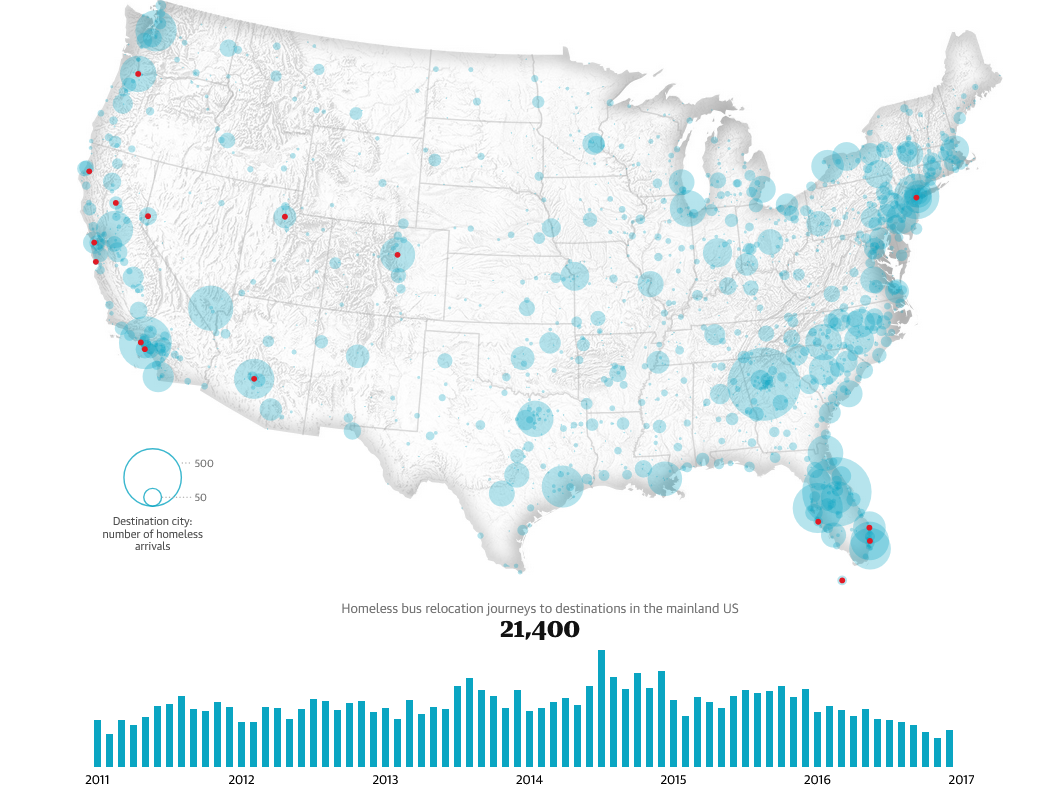
\includegraphics{homelessness_graph.png} \#\#Part A
The data behind the graph would be the homeless bus relocations in the
mainland United States over the period from 2011 to 2017. The rows would
the year and the columns would the total number of homeless bus
relocations to each city.

\#\#Part B Both columns would be numeric types as we are tracking
quantitative data and can count the total number of bus relocations.

\#\#Part C The data would be encoded by city since each city is given a
`circle' mark to indicate how many people relocated to the city via bus
during the time period. The marks would be derived from the number of
relocations and the circles follow a exponential scale of the total
number of relocations.

\#\#Part D Yes since we are given a map of the US to show visually what
cities were the most effected as well as a bar graph that gives a
general overview of the change in number of bus relocations over the
time period.

\end{document}
